\chapter{On the problem to set coverage obligations}
%\addcontentsline{toc}{section}{On the problem to set coverage obligations}
This chapter undertakes a detailed analysis of the problem to set coverage obligations. The first part analyses the most frequently used spectrum allocation mechanisms and the reasons why coverage obligations are normally used to force MNOs to provide a minimum broadband access speed. After that, I analyze all the parameters that define a coverage obligation set (Time frame, the scope, if it is only for data service or for data and voice service, etc.). Finally, I review the coverage obligations set for 800 MHz for Spain, the UK, Germany, and France to illustrate how these were set in one of the latest spectrum auctions.\par

\section{Mechanisms to allocate spectrum}
%\addcontentsline{toc}{subsection}{Mechanisms to allocate spectrum}
According to this document of the Spanish Ministry for the Digital Agenda (MINETAD) \cite{2-01}, there were several mechanisms to assign public spectrum to mobile operators in the past, namely:\par

\begin{itemize}
	\item Administrative grant: This allocation had no transparency nor quickness because it was the responsibility of the government to decide the frequency band, technology and other specifications of the service \cite{2-02}. In the UK, licenses were awarded for a specific technology and use and without raising interests until the 1998 Wireless Telegraphy Act \cite{2-06}]. This act enabled the usage of auctions to grant licenses and the first auction was in 2000 for 3G mobile licenses.\par

	\item Lottery: The spectrum is partitioned and given to the MNOs. This mechanism is transparent and quicker, although it is neither fair nor efficient because the allocation is not related to any technical factor. This mechanism was used in the distribution of the 3G spectrum in the U.S.\par

	\item Scoring rule: Using scoring rules, the government notify the set of factors that will weigh in the decision and the MNOs that are interested in the spectrum just send their applications. The decision is taken by the government, which can incur in lack of transparency.\par

	\item Auctions: This is a transparent and raising-oriented mechanism that became more popular since 2000 and 2001 when countries that created auctions to allocate the spectrum for 3G raised pretty much money than countries that used the traditional public competition.
\end{itemize}\par

Once spectrum is allocated, regulatory bodies must ensure that it is used in an effective and fair way, enforcing MNOs to invest nationwide and not only in the most cost-effective areas. Hence, policies should target primarily the least populated areas, where the cost of user capacity is higher. According to this GSMA report \cite{2-03}, there are three types of areas depending on their economic viability with regards to new mobile broadband rollout:\par

\begin{itemize}
	\item Type 1: Areas which will be covered by network competition.\par

	\item Type 2: Areas which can only be covered with network-sharing or a single network.\par

	\item Type 3: Areas which can only be covered with some form of public funding.
\end{itemize}\par

Regulators must focus their efforts on fostering the deployment of mobile broadband networks in areas of type 2 and 3. In the paper, GSMA also defines three main mechanisms regulators can make use of:\par

\begin{itemize}
	\item Tool 1: Promoting voluntary infrastructure sharing in rural areas.\par

	\item Tool 2: Licensing of low-frequency spectrum in combination with coverage obligations.\par

	\item Tool 3: Using public finances to (co)fund rollout in uneconomic rural areas.
\end{itemize}\par

Infrastructure sharing is a tool that is widely used in Europe due to the difference in the size of the companies in the telecom sector. Examples were the national roaming agreement in Spain between Yoigo and Vodafone since Yoigo’s coverage was limited to urban areas and the agreement between H3G and O2 in the UK. These GSMA report \cite{2-04} has a complete list of agreements in European countries.\par

According to the Florence School of Regulation [5], the third tool is not advised as they suggest that \textit{«simply reducing the immediate and direct cost of access to broadband connections through supply-side policies may not be enough to stimulate broadband subscriptions»}, since the perceived benefits from broadband access do not compensate the cost of the broadband connection for end-users. This tool seems to be interesting for the MNOs because they could reduce the CAPEX, but end users would not choose to pay for a broadband service that they would not use and, therefore, MNOs would not deploy new assets. \par

Therefore, only the second tool can help to truly stimulate mobile coverage in rural areas, due to the rollout of more mobile coverage is not subsidized but mandatory. This course of action will probably also foster end-users from rural areas to use mobile services.\par

The following figure, obtained from \cite{2-03}, shows the effect that adding coverage obligations have on the price of the spectrum. It can be considered as a priced reduction in exchange for promoting an obligatory inversion in new coverage for several years (until the threshold coverage is reached).

%%%%%%%%%%%%%%%%%%%% Figure/Image No: 8 starts here %%%%%%%%%%%%%%%%%%%%

\begin{figure}[H]
	\begin{Center}
		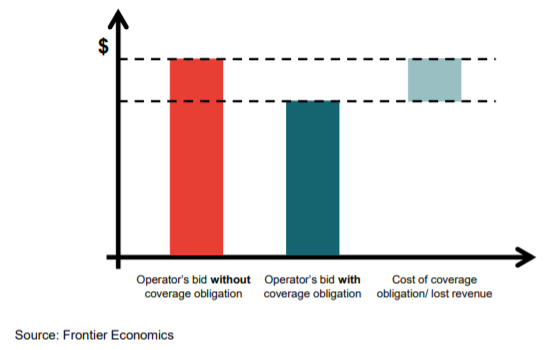
\includegraphics[width=0.95\textwidth]{./media/image8.png}
		\caption{Impact of the coverage obligations in the operator's bid \cite{2-03}}
	\end{Center}
\end{figure}


%%%%%%%%%%%%%%%%%%%% Figure/Image No: 8 Ends here %%%%%%%%%%%%%%%%%%%%
As an example, the UK spectrum allocation history is accurately explained in this publication of the parliament of the UK \cite{2-07}. Spain defined different coverage obligations for each spectrum band that has been allocated for mobile communications:\par
\begin{itemize}
	\item 800 MHz: 30 Mbit/s available to 90 $\%$  of citizens living in population centres of less than 5.000 inhabitants.\par

	\item 900 MHz: Population entities of less than 1000 inhabitants with a minimum level of -90dBm of UMTS 900 outdoor.\par

	\item 1800 MHz: Coverage obligation in cities higher than 500,000 inhabitants before 1999.\par

	\item 2100 MHz: Coverage obligation in cities higher than 250,000 inhabitants before 2003.\par

	\item 2600 MHz: No coverage obligations.
\end{itemize}\par

In March 2015, the ECC CEPT elaborated a big report about mobile coverage obligations \cite{2-08 which contains several classifications of the coverage obligations and answers that policymakers of 29 countries gave to a set of questions about their coverage obligations.  This report shows how widespread is the usage of coverage obligations at this time. According to the 29 countries in the survey:\par

\begin{itemize}
	\item 24 administrations have imposed coverage obligations regarding the voice service in one or more frequency bands;\par

	\item 25 administrations have imposed coverage obligations regarding the data service in one or more frequency bands.
\end{itemize}\par











\section{Defining coverage obligations}
%\addcontentsline{toc}{subsection}{Defining coverage obligations}
According to \cite{2-08} and \cite{2-03}, coverage obligations can be defined in multiple ways regarding several factors. All the examples in this section are answers that the countries submitted to the ECC CEPT questionnaire:\par

\begin{itemize}
	\item The object of study:\par

\begin{itemize}
	\item Population coverage: The operator needs to cover a percentage of the population.\par

	\item Area coverage: The operator needs to cover a percentage of the territory.\par

\end{itemize}
\end{itemize}
\begin{itemize}
	\item Timeframe:\par

\begin{itemize}
	\item Fixed in time: Certain percentage covered in certain years.\par

	\item Gradual through time: The percentage to cover grows every certain year.\par
\end{itemize}
\end{itemize}
For example, France «\textit{Gradual through time»} example will be studied in the following chapter and Belgium defined these three milestones: 30$\%$  of population 2 years after obtaining a license, 70$\%$  of population 4 years after obtaining a license and 98$\%$  of population 6 years after obtaining a license. In the opposite case, Spain and the UK defined just one milestone in 2020 and 2017 respectively.\par

\begin{itemize}
	\item Frequency band:\par

\begin{itemize}
	\item Using a specific band.\par

	\item Using any band allocated to the operator.\par

\end{itemize}
\end{itemize}
As an example, operators in Spain and Portugal can fulfil the data coverage obligations using any frequency band or technology allocated for mobile operators. On the contrary, each band has its own coverage obligation in France.\par


\begin{itemize}
	\item Spectrum’s blocks differentiation:\par

\begin{itemize}
	\item All blocks of the band have the same coverage obligations.\par

	\item Some blocks have more coverage obligations than others.\par
\end{itemize}
\end{itemize}
In Finland, there are two different coverage obligation sets in the 800 MHz frequency band, one has higher obligations compared to two other licenses: One mobile network has to cover 95 $\%$  of the population of mainland Finland within three years of the license period, and 99 $\%$  of the mainland of Finland's population within five years of the license period; two other mobile networks have to cover 97 $\%$  of the population of mainland Finland within five years of the license period begins.  Another example is the UK, where Ofcom offered one block of spectrum bigger than the others, but with data service coverage obligations. We will study this case later in this chapter \cite{2-09}.\par

\begin{itemize}
	\item The scope of the coverage obligation:\par

\begin{itemize}
	\item Each operator must fulfil the coverage obligation on their own.\par

	\item Coverage obligations are designed to be covered collaboratively.\par
\end{itemize}
\end{itemize}
When each spectrum’s block has different coverage obligations, they are usually enforced separately to each operator. This makes sense since if the distribution of the spectrum is not equal among all the operators, obligations must vary. However, the Spanish government allowed fulfilling the data coverage obligation rate using a combination of resources of all the available operators. The following chapter explains it extensively.\par

\begin{itemize}
	\item Area-specific obligations:\par

\begin{itemize}
	\item The coverage obligations affect all the territory equally.\par

	\item The country can be divided and coverage obligations are defined independently for each slice or only some areas are under specific coverage obligations.
\end{itemize}
\end{itemize}

Two examples will be explained later: the UK and the coverage obligation per nation and France and their $``$Area of high priority$"$ .\par

Once coverage obligations are defined, two more points have to be defined: the parameters that the policymaker will evaluate to check if the MNO has fulfilled the coverage obligations and which are the mechanisms that the policymakers will use to evaluate those parameters.\par

\subsection*{How to evaluate if the data coverage obligation is fulfilled:}
%\addcontentsline{toc}{subsubsection}{How to evaluate if the data coverage obligation is fulfilled:}
The questionnaire of ECC CEPT \cite{2-08} had also one question about the kind of criteria that defined that coverage obligations are fulfilled or not. Answers of the countries showed the following criteria:\par

\begin{itemize}
	\item Maximum theoretical data rate.\par

	\item Downlink data rate.\par

	\item Minimum of the population to be covered with a specific minimum data rate.\par

	\item Specific outdoor or indoor coverage.\par

	\item Limit values for RSRP (Reference Signal Received Power) and SINR (Signal-to-Interference-plus-Noise Ratio).
\end{itemize}\par

\subsection*{How to enforce telecom operators to meet coverage obligations}
%\addcontentsline{toc}{subsubsection}{How policymaker enforce telecom operators to meet coverage obligations}
There is no international plan, not even a European plan, to standardize the control of the growth of the coverage in the country. According to the questionnaire cited above, countries use three main strategies to control the coverage:\par

\begin{itemize}
	\item Regulators can use the information provided by the operators to verify the progress of the investments to increase the coverage in the country.\par

	\item If operators do not publish this information, regulators can use other information of the operators, such as the location of the base stations, antennas’ propagation model, network load, etc., to estimate the coverage theoretically.\par

	\item Finally, regulators can complement this information with some field measurements that validate the information supplied, but this is an expensive measure. It can be useful for some key areas and to validate the estimations made with the other strategies.
\end{itemize}\par















\section{Coverage obligations in the first digital dividend}
%\addcontentsline{toc}{subsection}{Coverage obligations in the first digital dividend}
The terms and conditions that telecom operators must follow to have access to the 800 MHz band depend on the country, but most of the European regulators included coverage obligations in the auctions. As everything suggests that the coverage obligations of the second dividend will be like the ones applied years ago, the first digital dividend will be analyzed.\par

\subsection*{Spain}
\addcontentsline{toc}{subsection}{Spain}
The Sustainable Economy Act of March 4, 2011 (Act 2/2011) \cite{2-10} established in the Article 51 that the 800MHz band was meant for advanced services for electronic communications and that it should be free to allocate before January 1, 2015. Regardless of what was said, it did not happen until April 1, 2015, because the Spanish Supreme Court declared that the channels of one TV multiplex where assigned without public competition \cite{2-12}.\par

MINETUR (The Industry, Tourism and Commerce ministry) decided that each of the spectrum blocks of the auction should have 5 MHz for uplink and downlink. Therefore, there were 6 blocks for each direction. According to this ministry \cite{2-11}, Vodafone, Orange – as France Telecom – and Telefónica got each of them, 2 blocks for uplink and 2 for downlink, dividing the spectrum equally between them. The block which was supposed to have more noise from the Terrestrial TV signals was assigned to Orange in exchange for paying less for it.


%%%%%%%%%%%%%%%%%%%% Figure/Image No: 9 starts here %%%%%%%%%%%%%%%%%%%%

\begin{figure}[H]
	\begin{Center}
		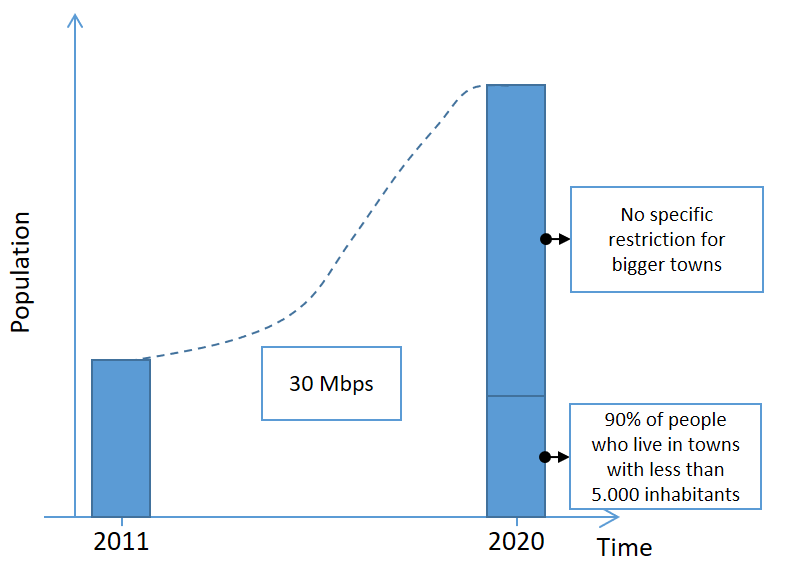
\includegraphics[width=0.95\textwidth]{./media/image9.png}
		\caption{Coverage obligations in Spain. Source: Author}
	\end{Center}
\end{figure}


%%%%%%%%%%%%%%%%%%%% Figure/Image No: 9 Ends here %%%%%%%%%%%%%%%%%%%%

According to what it is established in the article 6.2 of the Royal Decree 458/2011 (Spanish Official State Gazette of April 29, 2011), MINETUR established that those MNOs that have spectrum in the 800 MHz band have to create a joined plan to offer at least 30 Mbps to 90$\%$  of the inhabitants of population sizes smaller than 5,000 people before January 1, 2020.\par




\subsection*{The United Kingdom}
\addcontentsline{toc}{subsection}{The United Kingdom}
The policymaker responsible for defining the guidelines of the digital dividend in the United Kingdom was Ofcom. This public agency published on March 22, 2011, a consultation \cite{2-13} with the key conditions to request the MNOs. This consultation was about how Ofcom should award this new spectrum in a way that secures the best use for the benefit of citizens and consumers. In this consultation, the policymaker defined a spectrum auction with limits in the spectrum that each MNO can win:\par
\begin{itemize}
	\item Lower limits, defined as floors, are the minimum spectrum that an operator needs to be considered as a $``$credible national wholesaler$"$  in this situation. The auction would be valid if four or more operators end with at least one of the following options:\par

\begin{itemize}
	\item 2x5 MHz of sub-1 GHz and 2x20 MHz of 2.6 GHz; or
	\item 2x5 MHz of sub-1 GHz and 2x15 MHz of 1800 MHz; or
	\item 2x10 MHz of sub-1 GHz and 2x15 MHz of 2.6 GHz; or
	\item 2x10 MHz of sub-1 GHz and 2x10 MHz of 1800 MHz; or
	\item 2x15 MHz of sub-1 GHz.\par
\end{itemize}
	\item Upper limits, defined as caps, are the maximum amount of spectrum each participant could win in the auction. The caps were: 2x27.5 MHz of sub-1 GHz spectrum and 2x105 MHz of mobile spectrum in total.\par
\end{itemize}

Ofcom divided the available spectrum into blocks of 5 MHz, paired and with reverse duplex direction. This is illustrated in the figure below:



%%%%%%%%%%%%%%%%%%%% Figure/Image No: 10 starts here %%%%%%%%%%%%%%%%%%%%

\begin{figure}[H]
	\begin{Center}
		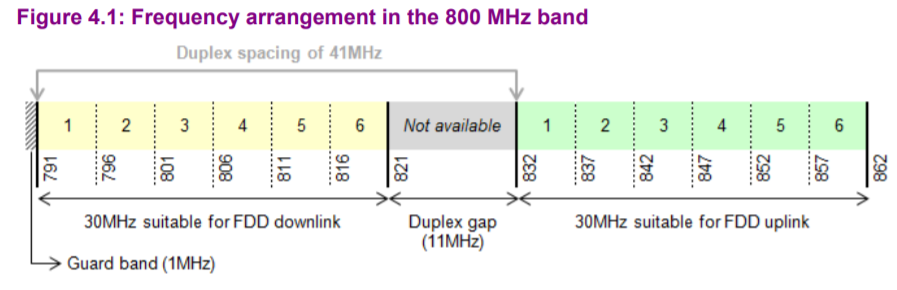
\includegraphics[width=1.00\textwidth]{./media/image10.png}
		\caption{Frequency arrangement in the UK in the 800 MHz band. Ofcom\cite{2-13}}
	\end{Center}
\end{figure}


%%%%%%%%%%%%%%%%%%%% Figure/Image No: 10 Ends here %%%%%%%%%%%%%%%%%%%%

Moreover, Ofcom required two types of coverage obligations:\par

First, a coverage obligation in only one license \textit{«for the 800 MHz spectrum to deploy a network capable of providing mobile telecommunication services with a sustained downlink speed of 2Mbps with a 90$\%$  probability of indoor reception to an area within which at least 95$\%$  of the UK population lives by the end of 2017»} and\textit{ «to provide a minimum level of indoor data coverage to 98$\%$  of all UK premises by 31 December 2017»}.



%%%%%%%%%%%%%%%%%%%% Figure/Image No: 11 starts here %%%%%%%%%%%%%%%%%%%%

\begin{figure}[H]
	\begin{Center}
		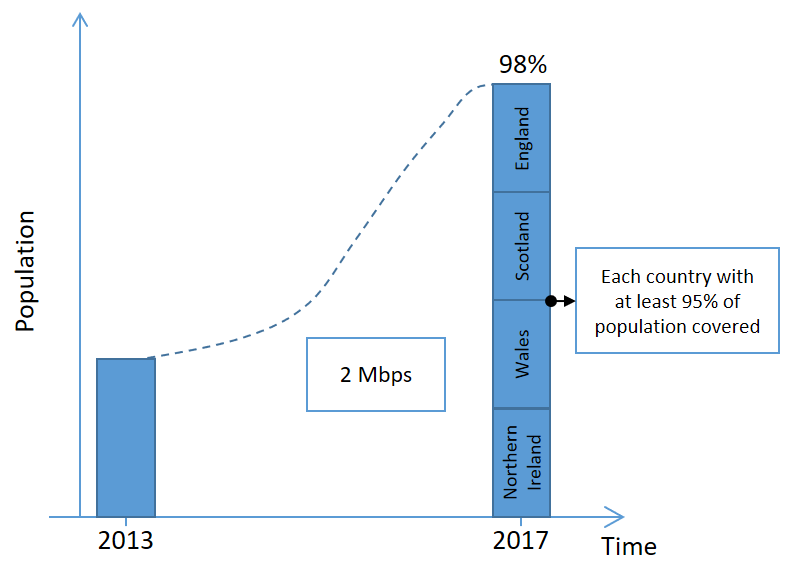
\includegraphics[width=0.80\textwidth]{./media/image11.png}
		\caption{Coverage obligations in the UK. Source: Author}
	\end{Center}
\end{figure}


%%%%%%%%%%%%%%%%%%%% Figure/Image No: 11 Ends here %%%%%%%%%%%%%%%%%%%%

Second, that \textit{$``$each MNO undertakes to enter into a binding commitment to implement 90 per cent geographic voice coverage throughout the UK by no later than 31 December 2017$"$ }. \par

This auction was held in 2013 and the results were public in March 2013 \cite{2-14}. Prices are not shown in the following table since the auction was of 800 MHz and 2600 MHz spectrum and Ofcom has not published disaggregated prices for each spectrum band.


%%%%%%%%%%%%%%%%%%%% Table No: 3 starts here %%%%%%%%%%%%%%%%%%%%


\begin{table}[H]
 			\centering

\begin{tabular}{p{1.42in}p{1in}p{1.36in}p{1.48in}}
\hline
%row no:1
\multicolumn{1}{|p{1.42in}}{\textbf{Licensee}} & 
\multicolumn{1}{|p{1in}}{\textbf{Number of blocks}} & 
\multicolumn{1}{|p{1.36in}}{\textbf{Frequencies}} & 
\multicolumn{1}{|p{1.48in}|}{\textbf{Coverage Obligations}} \\
\hhline{----}
%row no:2
\multicolumn{1}{|p{1.42in}}{Everything Everywhere Limited} & 
\multicolumn{1}{|p{1in}}{1 Uplink \par 1 Downlink} & 
\multicolumn{1}{|p{1in}}{796 to 801 MHz \par 837 to 842 MHz} & 
\multicolumn{1}{|p{1.48in}|}{Voice coverage} \\
\hhline{----}
%row no:3
\multicolumn{1}{|p{1.42in}}{Hutchison 3G \par UK Limited} & 
\multicolumn{1}{|p{1in}}{1 Uplink \par 1 Downlink} & 
\multicolumn{1}{|p{1.36in}}{791 to 796 MHz \par 832 to 837 MHz} & 
\multicolumn{1}{|p{1.48in}|}{Voice coverage} \\
\hhline{----}
%row no:4
\multicolumn{1}{|p{1.42in}}{Telefónica UK \par Limited} & 
\multicolumn{1}{|p{1in}}{2 Uplink \par 2 Downlink} & 
\multicolumn{1}{|p{1.36in}}{811 to 821 MHz \par 852 to 862 MHz} & 
\multicolumn{1}{|p{1.48in}|}{Voice coverage + \par Data coverage obligation} \\
\hhline{----}
%row no:5
\multicolumn{1}{|p{1.42in}}{Vodafone \par Limited} & 
\multicolumn{1}{|p{1in}}{2 Uplink \par 2 Downlink} & 
\multicolumn{1}{|p{1.36in}}{801 to 811 MHz \par 842 to 852 MHz} & 
\multicolumn{1}{|p{1.48in}|}{Voice coverage} \\
\hhline{----}

\end{tabular}
\caption{Results of the spectrum auction in the UK in 2013. Ofcom \cite{2-14}}

 \end{table}


%%%%%%%%%%%%%%%%%%%% Table No: 3 ends here %%%%%%%%%%%%%%%%%%%%

Telefónica UK was the MNO that was required, under the terms of its 4G/800 MHz license to provide both data coverage obligations. Terms and conditions that measure the compliance with these obligations are detailed in \cite{2-15} for voice coverage and in \cite{2-16} for data coverage obligation.\par

Finally, on 9\textsuperscript{th} March 2018, Ofcom sent letters to all operators confirming the compliance of the conditions mentioned before \cite{2-17}.\par

\subsection*{France}
\addcontentsline{toc}{subsection}{France}
Arcep (\textit{Autorité de regulation des communications électroniques et des Postes}) is the body responsible for regulating telecommunications in France \cite{2-18}. Arcep fixes general obligations that operators must meet, imposes penalties for those that do not fulfil the obligations, sets the amount of money that has to be paid in exchange for spectrum allocations and allocates frequency bands. Despite Arcep is the agency that allocates bands for MNOs, the ANFR (\textit{Agence Nationale des fréquences}) is the organization with the competence of defining the service that is allocated to each spectrum band \cite{2-19}.\par

After the approval of the French parliament, Arcep announced on May 2011 the procedures for allocating the frequencies for deploying 4G: 800 MHz band \cite{2-20} and 2600 MHz band \cite{2-21}. According to \cite{2-22}, Arcep defined three goals to achieve with the allocation of these bands:\par

\begin{itemize}
	\item Digital regional development. The Pintat Act of December 17, 2009 \cite{2-23}, set as a top priority the reduction of the digital break and to work towards that, Arceparcep defined three types of coverage obligations for each carrier:\par

\begin{itemize}
	\item To cover 99.6$\%$  of the population of mainland France before 2027.\par

	\item To cover 95$\%$  of the population of each department of mainland France before 2027.\par

	\item To cover 90$\%$  of the priority areas before 2022. The priority area comprises the most sparsely populated regions of mainland France (63$\%$  of the surface area, but only 18$\%$  of the population of France). The full list of almost 95.627 towns can be checked using the following link \cite{2-24}.\par

	\item All previous obligations had several intermediate milestones that can be checked in the figure below.



%%%%%%%%%%%%%%%%%%%% Figure/Image No: 12 starts here %%%%%%%%%%%%%%%%%%%%

\begin{figure}[H]
	\begin{Center}
		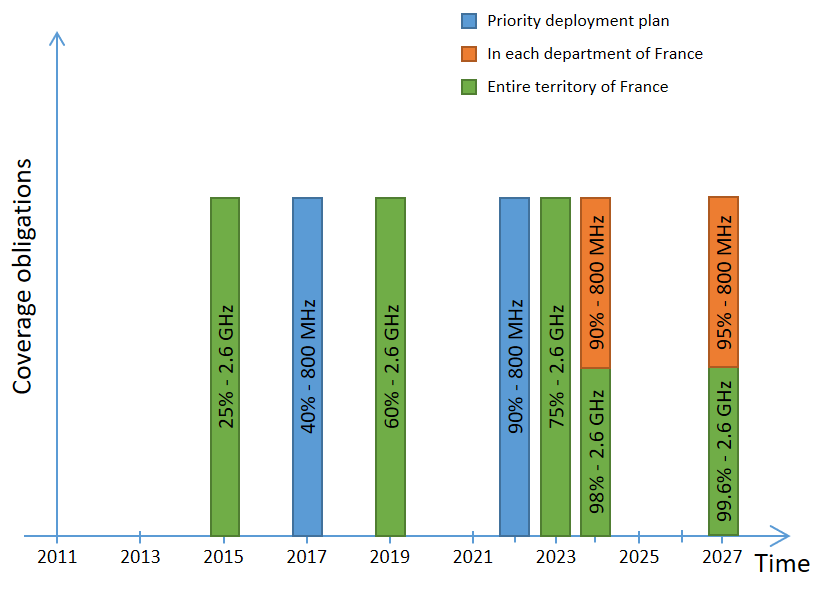
\includegraphics[width=0.95\textwidth]{./media/image12.png}
		\caption{Coverage obligations in France. Source: Author}
	\end{Center}
\end{figure}


%%%%%%%%%%%%%%%%%%%% Figure/Image No: 12 Ends here %%%%%%%%%%%%%%%%%%%%

\end{itemize}
	\item Ensure fair and effective competition in the mobile market. \textit{«the amount of spectrum that any operator will be awarded cannot exceed a 15 MHz duplex in the 800 MHz band and a 30 MHz duplex in the 2.6 GHz band. Moreover, should there be four eligible candidates for the 2.6 GHz-band frequencies, each carrier is guaranteed to receive a 15 MHz duplex if it has applied for this quantity of spectrum»}\par

	\item The proper monetization of the spectrum. To do so, the amount that candidates bid was a key criterion to win the spectrum band and each band had a minimum price to bid.
\end{itemize}\par

After the spectrum auction, Arcep published on December 22, 2011, the results of the awards procedure \cite{2-25}. These are the MNOs that won part of the spectrum:



%%%%%%%%%%%%%%%%%%%% Table No: 4 starts here %%%%%%%%%%%%%%%%%%%%


\begin{table}[H]
 			\centering
\caption{Results of the spectrum auction in France in 2011. Arcep \cite{2-25}}

\begin{tabular}{p{1.35in}p{1.35in}p{1.35in}}
\hline
%row no:1
\multicolumn{1}{|p{1.35in}}{\textbf{License recipient}} & 
\multicolumn{1}{|p{1.35in}}{\textbf{Spectrum awarded}} & 
\multicolumn{1}{|p{1.35in}|}{\textbf{Financial bid}} \\
\hhline{---}
%row no:2
\multicolumn{1}{|p{1.35in}}{Bouygues Telecom} & 
\multicolumn{1}{|p{1.35in}}{10 MHz duplex} & 
\multicolumn{1}{|p{1.35in}|}{683,087,000€} \\
\hhline{---}
%row no:3
\multicolumn{1}{|p{1.35in}}{SFR} & 
\multicolumn{1}{|p{1.35in}}{10 MHz duplex} & 
\multicolumn{1}{|p{1.35in}|}{1,065,000,000€} \\
\hhline{---}
%row no:4
\multicolumn{1}{|p{1.35in}}{Orange France} & 
\multicolumn{1}{|p{1.35in}}{10 MHz duplex} & 
\multicolumn{1}{|p{1.35in}|}{891,000,005€} \\
\hhline{---}

\end{tabular}
 \end{table}


%%%%%%%%%%%%%%%%%%%% Table No: 4 ends here %%%%%%%%%%%%%%%%%%%%

\subsection*{Germany}
\addcontentsline{toc}{subsection}{Germany}
In Germany, the policymaker responsible for regulating the telecommunication spectrum is the Bundesnetzagentur \cite{2-26} and is a federal government agency part of the German Federal Ministry of Economics and Technology (BMWi). Its main duties are the promotion of telecommunications services in public institutions, the administration of frequencies and phone numbers and the resolution of radio interferences.\par

Even though it is a national institution, Germany’s federal structure allows each federal state (Bundesland) to share some competences with the Bundesnetzagentur. Each Bundesland is responsible for regulating spectrum capacities for broadcasting purposes in its region, but the allocation of the broadcasting frequencies and the assignment process on request of capacities by the Bundesländer (plural) are a task of the national regulatory authority.\par

The process of the allocation of the 800 MHz band started on 18 February 2009, when the German Federal Cabinet announced its broadband strategy, which included a focus on making broadband access more widely available in rural areas \cite{2-27}.  After that, the Bundesrat, which is the body that represents both the Federal government and the Bundesländer, approved the Federal Cabinet decision \cite{2-28}. Finally, Bundesnetzagentur published the requirements and conditions for the allocation of the spectrum \cite{2-29}.\par

The spectrum auction started on 12 April 2010 and ended on 20 May 2010 and offered spectrum blocks from several bands:\par

\begin{itemize}
	\item 6 blocks of 2x5 MHz paired in the 800 MHz band.\par

	\item 5 blocks of 2x5 MHz paired in the 1800 MHz band.\par

	\item 8 blocks of 2x4.9 MHz paired in the 2 GHz band.\par

	\item 19.2 MHz unpaired in the 2 GHz band.\par

	\item 14 blocks of 2x5 MHz paired in the 2.6 GHz band.\par

	\item 10 blocks of 2x5 MHz unpaired in the 2.6 GHz band.
\end{itemize}\par

This auction also included significant coverage obligations only for the telecom operators that won some spectrum in the 800 MHz. Administrations of each Bundesländer defined the so-called $``$Weiße Flecken-Listen$"$  (white spot lists) and categorized villages in each Bundesland into four priority levels. For a complete list of villages for each priority and Bundesland check the following link \cite{2-30}. This way, each telecom operator can only increase the capacity of its network in an area if it has covered at least 90$\%$  of the population of the areas of the higher priority. Such connections were defined as having transmission rates of at least 1 Mbps, but due to the technical difficulties to measure a real mean download speed, the final condition is just to provide the mobile broadband connection.\par



%%%%%%%%%%%%%%%%%%%% Table No: 5 starts here %%%%%%%%%%%%%%%%%%%%


\begin{table}[H]
 			\centering
\caption{Conditions of the spectrum auction in Germany in 2010. German's Bundesnetzagentur \cite{2-30}}

\begin{tabular}{p{1in}p{2.3in}p{2in}}
\hline
%row no:1
\multicolumn{1}{|p{1in}}{\Centering \textbf{STAGE}} & 
\multicolumn{1}{|p{2.3in}}{\Centering \textbf{POPULATION SIZE}} & 
\multicolumn{1}{|p{1.7in}|}{\Centering \textbf{MIN. COVERAGE}} \\
\hhline{---}
%row no:2
\multicolumn{1}{|p{1in}}{\Centering Priority 1} & 
\multicolumn{1}{|p{2.3in}}{\Centering < 5,000 inhabitants} & 
\multicolumn{1}{|p{1.7in}|}{\Centering 90$\%$ } \\
\hhline{---}
%row no:3
\multicolumn{1}{|p{1in}}{\Centering Priority 2} & 
\multicolumn{1}{|p{2.3in}}{\Centering > 5,000 inhabitants \par \Centering < 20,000 inhabitants} & 
\multicolumn{1}{|p{1.7in}|}{\Centering 90$\%$ } \\
\hhline{---}
%row no:4
\multicolumn{1}{|p{1in}}{\Centering Priority 3} & 
\multicolumn{1}{|p{2.3in}}{\Centering > 20,000 inhabitants \par \Centering < 50,000 inhabitants} & 
\multicolumn{1}{|p{1.7in}|}{\Centering 90$\%$ } \\
\hhline{---}
%row no:5
\multicolumn{1}{|p{1in}}{\Centering Priority 4} & 
\multicolumn{1}{|p{2.3in}}{\Centering > 50,000 inhabitants} & 
\multicolumn{1}{|p{1.7in}|}{\Centering 90$\%$ } \\
\hhline{---}

\end{tabular}
 \end{table}


%%%%%%%%%%%%%%%%%%%% Table No: 5 ends here %%%%%%%%%%%%%%%%%%%%

The following chart represents the allocation made in the spectrum auction of 2010. In the 800 MHz band, three operators won spectrum: Deutsche Telekom, Telefónica O2, and Vodafone. All of them received the same amount of spectrum and the same coverage obligations.


%%%%%%%%%%%%%%%%%%%% Figure/Image No: 13 starts here %%%%%%%%%%%%%%%%%%%%

\begin{figure}[H]
	\begin{Center}
		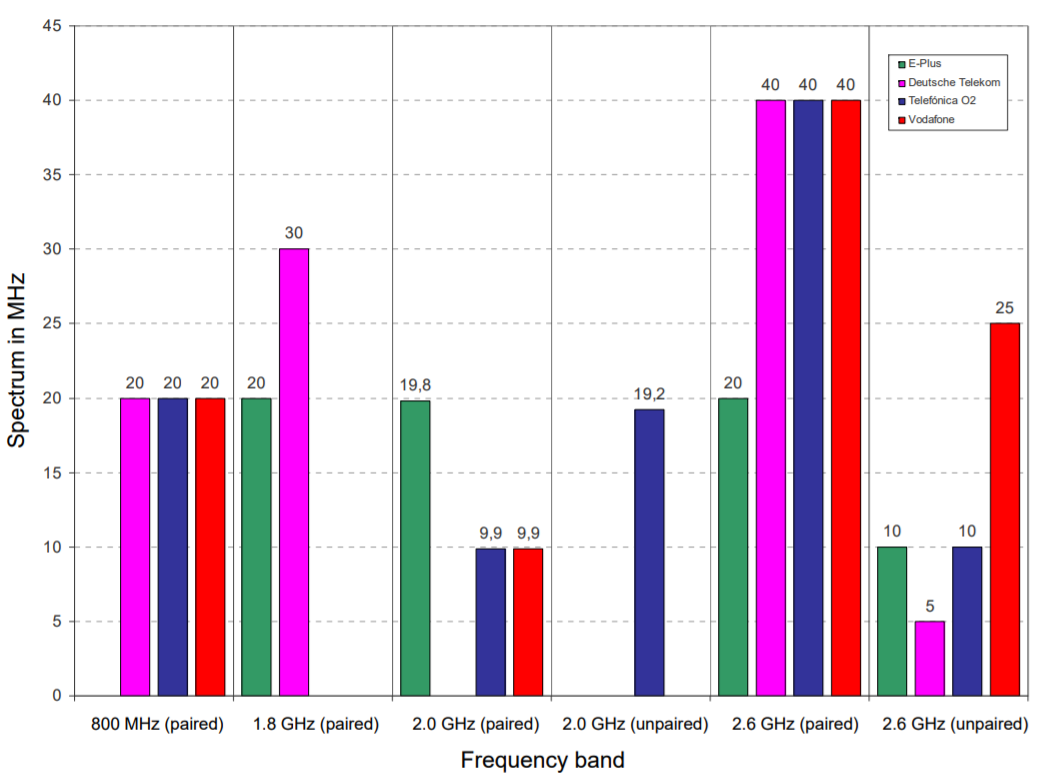
\includegraphics[width=0.95\textwidth]{./media/image13.png}
		\caption{Allocation of spectrum in the German auction of 2010. German's Bundesnetzagentur\cite{2-32}}
	\end{Center}
\end{figure}

%%%%%%%%%%%%%%%%%%%% Figure/Image No: 13 Ends here %%%%%%%%%%%%%%%%%%%%

Finally, on 26 November 2012, the Bundesnetzagentur announced that \textit{«The mobile phone companies have now fulfilled the coverage obligations in the 800 MHz range. The three companies Telekom Deutschland, Vodafone and Telefónica Germany can now freely use the frequencies they have purchased in the 800 MHz band in all federal states»} \cite{2-31}.\par
